\documentclass{article}
\usepackage{graphicx} % Required for inserting images
\usepackage{amsmath}
\usepackage{matlab-prettifier}

\title{Project Part 2: One-Dimensional Tracking Simulation Contstruction}
\author{Devin Smith \\ UIN: 330000494}
\date{Applied Kalman Filtering\\AERO 689-603}

\begin{document}

\maketitle

\section{Problem Statement}
Begin the development of the simulation of the continuous-time dynamics of the falling body with
discrete-time measurements of range. Recall the mathematical models for the one-dimensional tracking problem form Part 1, illustrated in Figure 1. The tracking problem simulation is shown in Figure 2.

\begin{figure}[h]
    \centering
    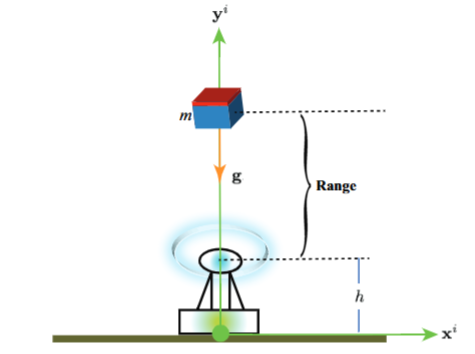
\includegraphics[width=1\linewidth]{Figure_1.png}
    \caption{One-Dimensional tracking problem scenario}
    \label{fig:enter-label}
\end{figure}

\begin{figure}[h]
    \centering
    \includegraphics[width=1\linewidth]{Figure_2.png}
    \caption{Simulation tracking diagram}
    \label{fig:enter-label}
\end{figure}

\subsection{Assumptions}

\begin{enumerate}
    \item Gravity, \textbf{$g$}, and height, \textit{$h$} are known constants
    \item Atmospheric drag is neglected
    \item Motion is one-dimentional (along the \textbf{$y^i$} axis)
    \item Range measurements (measured from the radar antennae dish - not the ground) are available at discrete times
\end{enumerate}

\subsection{Tasks}

\begin{enumerate}
    \item Using the state-space model developed in Part 1, create a simulation to numerically integrate the equations of motion of the falling body with constant gravity and process noise and generate noisy discrete-time range measurements. Be sure to adequately comment your code.
    \item The inputs of the simulation are
    \begin{itemize}
        \item Initial state, $x_0 = \begin{bmatrix}
            \underline{r}_0 \\ \underline{v}_0
        \end{bmatrix}$
        \item Process noise $Q_s = \begin{bmatrix} 0 & 0 & 0 & 0 \\ 0 & 0 & 0 & 0 \\ 0 & 0 & 0 & 0 \\ 0 & 0 & 0 & q_s 
        \end{bmatrix}$
        \item Measurement Noise $R_k$
        \item Measurement update rate $\Delta t_k$
        \item Height above the ground $h$
    \end{itemize}
    \item Consider the following values $r_0 = \begin{bmatrix}
        0 \\ 1000
    \end{bmatrix} m$, $v_0 = \begin{bmatrix}
        0 \\ 0
    \end{bmatrix} m/s^2$, $h = 2$ m, $q_s = 0.01$ $m^2/s^5$, and $\Delta t_k = 0.5$ s 
\end{enumerate}

\section{Problem Formulation}

\subsection{Continuous-Time Model}
Recall the continuous-time state-space mathematical equations derived in part 1 of the one-dimensional tracking problem.

\subsubsection{Dynamics}

\begin{equation}
    \underline{\dot{r}}(t) = \underline{v}(t)
\end{equation}
\begin{equation}
    \underline{\ddot{r}}(t) = \underline{\dot{v}}(t) = -\underline{g}
\end{equation}

\begin{equation}
    \underline{\dot{x}}(t) = \mathbf{F}(t)\underline{x}(t) + \mathbf{G}(t)\underline{u}(t) + \underline{w}(t)
\end{equation}

\begin{equation*}
    \begin{bmatrix} \dot{r_x}(t) \\ \dot{r_y}(t) \\ \dot{v_x}(t) \\ \dot{v_y}(t) \end{bmatrix} = 
    \begin{bmatrix} 0 & 0 & 1 & 0 \\ 0 & 0 & 0 & 1 \\ 0 & 0 & 0 & 0 \\ 0 & 0 & 0 & 0 \end{bmatrix}
    \begin{bmatrix} r_x(t)\\r_y(t)\\v_x(t)\\v_y(t) \end{bmatrix} +
    \begin{bmatrix} 0 & 0 \\ 0 & 0 \\ 0 & 0 \\ 0 & 1 \end{bmatrix}
    \begin{bmatrix} 0\\-g \end{bmatrix} +
    \begin{bmatrix}
        0 \\ 0 \\ 0 \\ w(t)
    \end{bmatrix}
\end{equation*}

\begin{equation*}
    E\{\underline{w}(t)\} = \underline{0}
\end{equation*}
\begin{equation*}
    E\{\underline{w}(t)\underline{w}(\tau)^T\} = \mathbf{Q}_s(t)\delta(t-\tau), \forall t,\tau
\end{equation*}
\begin{equation*}
    \mathbf{Q}_s = 
    \begin{bmatrix} 0 & 0 & 0 & 0 \\ 0 & 0 & 0 & 0 \\ 0 & 0 & 0 & 0 \\ 0 & 0 & 0 & q_s \end{bmatrix}
\end{equation*}

\begin{equation*}
    \underline{x}_0 = \begin{bmatrix}
            \underline{r}_0 \\ \underline{v}_0
        \end{bmatrix}
\end{equation*}

\subsection{Discrete-Time Model}
Recall the discrete-time state-space mathematical equations derived in part 1 of the one-dimensional tracking problem.

\subsubsection{Dynamics}

\begin{equation}
    \underline{x}_k = \boldsymbol{\phi}_\mathrm{k-1}\underline{x}_\mathrm{k-1} + \underline{u}_\mathrm{k-1} + \underline{w}_\mathrm{k-1}
\end{equation}

\begin{equation}
    \boldsymbol{\phi}(t_k,t_\mathrm{k-1}) = e^{\mathbf{F}(t_k - t_\mathrm{k-1})}
\end{equation}

\begin{equation}
    \underline{u}_\mathrm{k-1} = \int_{t_\mathrm{k-1}}^{t_k} \boldsymbol{\phi}(t_k, \tau)\mathbf{G}(\tau)\underline{u}(\tau)d\tau
\end{equation}

\begin{equation*}
    \begin{bmatrix} 0 \\ r_k \\ 0 \\ v_k \end{bmatrix} = 
    \begin{bmatrix}
        1 & 0 & \Delta t & 0\\
        0 & 1 & 0 & \Delta t \\
        0 & 0 & 1 & 0 \\
        0 & 0 & 0 & 1
    \end{bmatrix}
    \begin{bmatrix} 0\\r_\mathrm{k-1}\\0\\v_\mathrm{k-1} \end{bmatrix} - g
    \begin{bmatrix}
        0 \\
        \dfrac{{\Delta t}^2}{2} \\
        0 \\
        \Delta t
    \end{bmatrix}
    +
    \underline{w}_\mathrm{k-1}
\end{equation*}

\begin{equation}
    \underline{w}_\mathrm{k-1} = \int_{t_\mathrm{k-1}}^{t_k} \boldsymbol{\phi}(t_k, \tau)\underline{w}(\tau)d\tau
\end{equation}

\begin{equation}
    E\{\underline{w}_\mathrm{k-1}\} = \int_{t_\mathrm{k-1}}^{t_k} \boldsymbol{\phi}(t_k, \tau)E\{\underline{w}(\tau)\}d\tau = \underline{0}
\end{equation}

\begin{equation}
    E\{\underline{w}_\mathrm{k-1}\underline{w}_\mathrm{k-1}^T\} = \mathbf{Q}_\mathrm{k-1} = 
    \int_{t_\mathrm{k-1}}^{t_k} \boldsymbol{\phi}(t_k, \tau)\mathbf{Q}_s(\tau)\boldsymbol{\phi}^T(t_k, \tau)d\tau
\end{equation}

\begin{equation*}
    \mathbf{Q}_\mathrm{k-1} = q_s
    \begin{bmatrix}
        0 & 0 & 0 & 0\\
        0 & \dfrac{{\Delta t}^3}{3} & 0 & \dfrac{{\Delta t}^2}{2} \\
        0 & 0 & 0 & 0 \\
        0 & \dfrac{{\Delta t}^2}{2} & 0 & \Delta t
    \end{bmatrix}
\end{equation*}

\subsubsection{Measurements}

\begin{equation}
    \underline{y}_k = \underline{r}_k + \underline{b}
\end{equation}

\begin{equation}
    \underline{y}_k = \mathbf{H}\underline{x}_k + \underline{b} + \underline{v}_k
\end{equation}

\begin{equation*}
    y_k = 
    \begin{bmatrix}
        0 & 1 & 0 & 0
    \end{bmatrix}
    \begin{bmatrix} r_{x_k} \\r_{y_k} \\v_{x_k} \\v_{y_k} \end{bmatrix} - h + \nu_k
\end{equation*}

\begin{equation*}
    E\{\nu_k\} = 0
\end{equation*}

\begin{equation*}
    E\{\nu_k \nu_j\} = R_k\delta_kj
\end{equation*}

\section{Simulation}
Using the simulation diagram in Figure 2 and the desired user inputs from section 1.2, a simulation of the environment was created in MATLAB. This simulation contains several functions which take in the user inputs and simulate the falling object with process and measurement noise. The structure of the simulation is as follows:

\begin{enumerate}
    \item User inputs are defined.
    \item Generate a discrete-time state-space model of the dynamics (using a simulation time step). Generate a discrete-time state-space model of the measurements (using the measurement sampling rate).
    \item Initialize the states, process noise, measurement noise, and radar measurement at $t=0$.
    \item Simulate the environment until the object falls below the radar dish.
    \begin{itemize}
        \item Generate process noise and map discretized dynamics forward.
        \item Generate measurement noise and discretely measure range.
        \item Check if object is below radar.
    \end{itemize}
    \item Plot the states, measurements, process noise, and measurement noise.
\end{enumerate}

\par The results of the simulation with defined user inputs in section 1.2 are shown in Figures 3-8.

\begin{figure}[h]
    \centering
    \includegraphics[width=.8\linewidth]{Fig_3.png}
    \caption{True position vs time}
    \label{fig:enter-label}
\end{figure}

\begin{figure}[h]
    \centering
    \includegraphics[width=.8\linewidth]{Fig_4.png}
    \caption{True velocity vs time}
    \label{fig:enter-label}
\end{figure}

\begin{figure}[h]
    \centering
    \includegraphics[width=.8\linewidth]{Fig_5.png}
    \caption{Process noise vs time}
    \label{fig:enter-label}
\end{figure}

\begin{figure}[h]
    \centering
    \includegraphics[width=.8\linewidth]{Fig_6.png}
    \caption{Range measurements vs time}
    \label{fig:enter-label}
\end{figure}

\begin{figure}[h]
    \centering
    \includegraphics[width=.8\linewidth]{Fig_7.png}
    \caption{Measurement noise vs time}
    \label{fig:enter-label}
\end{figure}

\clearpage

\section{Summary}

Under the assumptions described in Section 1.1, the one-dimensional tracking model can be represented with both continuous-time and discrete-time state-space models of the dynamics, as well as a discrete-time model of the measurements. Equations 1-11 contain the equations for the continuous-time and discrete-time models. Using Figure 2 and the desired user inputs, a simulation was made for the environment of the dynamics and measurements. Figures 3-7 showcase the results of the simulation for the given numerical values for the problem in Section 1.2.
\par
With these mathematical models, the linear dynamics and measurements can be simulated with process and measurement noise. In later parts of the problem, the models will be modified with two-dimensional motion, filtering, and eventually non-linear dynamics and additional filtering methods. 

\section{Appendix: MATLAB Code}

\subsection{inp\_sim.m}
\begin{lstlisting}[style=Matlab-editor]
clear; clc; close all;

%% USER INPUT

% initial condition
inp.r0 = [0; 1000];     % [m] initial position
inp.v0 = [0; 0];        % [m/s] initial velocity

% sensor properties
inp.h = 2;              % [m] height of radar
inp.R = 4;              % [m^2] noise covariance
inp.mt = 0.5;           % [s] measurement sampling period

% process noise properties
inp.qs = .01;           % [m^2 / s^5] spectral density
inp.Qs = [0 0 0 0       % [m^2 / s^5] spectral density matrix
          0 0 0 0 
          0 0 0 0
          0 0 0 inp.qs];

%% SIMULATION

dt = 0.01;
plot_data = 1;
simulation(inp, dt, plot_data);
\end{lstlisting}

\subsection{simulation.m}
\begin{lstlisting}[style=Matlab-editor]
function simulation(inp, dt, plot_data)
%SIMULATION Simulates the entire falling object problem (part 2)
%   Creates state space model, and simulates the dynamcis + measurements.
%   Plots the data.

% set default parameters
if nargin < 2; dt = 0.01;   end
if nargin < 3; plot_data = 1; end

% get state space parameters
ss = state_space(inp, dt);

% initialize the state
state = initial_state(inp, ss);
state_hist = state;

% loop through the simulation
i = 1;
while state.falling
    state = env_sim(state, inp, dt, i, ss);
    state_hist = [state_hist, state];
    i = i + 1;
end

% pull stored data
r_hist = [state_hist.r];
v_hist = [state_hist.v];
t_hist = [state_hist.t];
w_hist = [state_hist.w];
nu_hist = unique([state_hist.nu]',"rows", "stable")';
y_hist = unique([state_hist.y]',"rows", "stable")';
tk_hist = unique([state_hist.tk]', "rows", "stable")';

% plot the stored data
if plot_data
    tmin = t_hist(1); tmax = t_hist(end);
    figure; plot(t_hist,r_hist(2,:)); xlim([tmin, tmax]);
    title("True Position"); xlabel("t (s)"); ylabel("r_y (m)");
    figure; plot(t_hist,v_hist(2,:)); xlim([tmin, tmax]);
    title("True Velocity"); xlabel("t (s)"); ylabel("v_y (m/s)");
    figure; hold on; xlim([tmin, tmax]);
    plot(t_hist, t_hist*0, 'k');
    plot(t_hist, ones(length(t_hist),1)*ss.Qk1(4,4), '--k');
    plot(t_hist, -ones(length(t_hist),1)*ss.Qk1(4,4), '--k');
    plot(t_hist,w_hist(4,:)); hold off;
    title("Process Noise"); xlabel("t (s)"); ylabel("w (m/s^2)");
    figure; plot(tk_hist,y_hist, 'x'); xlim([tmin, tmax]);
    title("Range Measurements"); xlabel("t (s)"); ylabel("y (m)");
    figure; hold on; xlim([tmin, tmax]);
    plot(t_hist, t_hist*0, 'k');
    plot(t_hist, ones(length(t_hist),1)*sqrt(inp.R), '--k');
    plot(t_hist, -ones(length(t_hist),1)*sqrt(inp.R), '--k');
    plot(tk_hist,nu_hist, 'x'); hold off;
    title("Measurement Noise"); xlabel("t (s)"); ylabel("nu (m)");
end
end

\end{lstlisting}

\subsection{state\_space.m}
\begin{lstlisting}[style=Matlab-editor]
function ss = state_space(inp, dt)
%STATE_SPACE Summary of this function goes here
%   Detailed explanation goes here

% definte the continuous dynamics
syms delt;          % symbolic delta t
g = 9.8066;         % [m/s^2] gravitational acceleration
u = [0; -g];
F = [0 0 1 0; 0 0 0 1; 0 0 0 0; 0 0 0 0];
G = [0 0; 0 0; 0 0; 0 1];

% calculate the discretized dynamics
phi = expm(F*(delt));                           % phi (symbolically)
Qk1 = double(int(phi*inp.Qs*phi',delt,0,dt));       % Q_k-1
Qk1 = [Qk1(2,2), Qk1(2,4); Qk1(4,2), Qk1(4,4)];
Qk1 = sqrtm(Qk1);

% get finalized discrete state space stuff
ss.uk1 = double(int(phi*G*u,delt,0, dt));          % u_k-1
ss.phi = expm(F*(dt));                             % phi (numerically)
ss.Qk1 = [0, 0, 0, 0; 0, Qk1(1,1), 0, Qk1(1,2); 
          0, 0, 0, 0; 0 Qk1(2,1), 0, Qk1(2,2)];
ss.H = [0 1 0 0];
ss.b = -inp.h;
ss.R = inp.R;
end
\end{lstlisting}

\subsection{initial\_state.m}
\begin{lstlisting}[style=Matlab-editor]
function ss = state_space(inp, dt)
function state = initial_state(inp, ss)
%INITIAL_STATE Creates the initial state, time, and process noise
state.r = inp.r0;                           % pull r0
state.v = inp.v0;                           % pull v0
state.t = 0;                                % let t0 = 0
state.w = [0; 0; 0; sqrt(inp.qs)]*randn;    % generate an initial w0
state = measure(state, ss);                 % get initial measurement
state.falling = true;
end
\end{lstlisting}

\subsection{measure.m}
\begin{lstlisting}[style=Matlab-editor]
function state = measure(state, ss)
%MEASURE Measures the position using the radar
%   yk = Hxk + b + nu_k

x = [state.r; state.v];         % pull current state

% simulate the measurements
nu = randn*sqrt(ss.R);          % generate measurement noise
y = ss.H*x + ss.b + nu;         % measure the state

% store the data
state.y = y;
state.tk = state.t;
state.nu = nu;

end
\end{lstlisting}

\subsection{env\_sim.m}
\begin{lstlisting}[style=Matlab-editor]
function state = env_sim(state, inp, dt, i, ss)
%ENVIRONMENT Simulates dynamics and measurements

% dynamics
state = dynamics(dt, state, ss);

% measurements
if rem(i,inp.mt/dt) == 0
    state = measure(state, ss);
end 

% check if above radar dish
if state.r(2) <= inp.h
    state.falling = false;
end
end
\end{lstlisting}

\subsection{dynamics.m}
\begin{lstlisting}[style=Matlab-editor]
function state = dynamics(dt, state, ss)
%DYNAMICS Simulates the dynamics
%   x_k1 = phi*xk + uk1 + wk1

x = [state.r; state.v]; % pull state

% simulate the dynamics
w = ss.Qk1*(randn(4,1));                      % process noise 
x = ss.phi*x + ss.uk1;                                % update x_k

% store the data
state.r = x(1:2);
state.v = x(3:4);
state.w = w;
state.t = state.t + dt;
end
\end{lstlisting}

\end{document}
